\documentclass[tikz,border=10pt]{standalone}
\usepackage{tikz}

\begin{document}

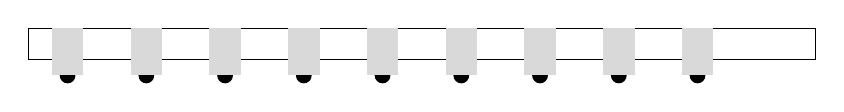
\begin{tikzpicture}[scale=2]

% Draw the white wall
\draw[fill=white] (0,0) rectangle (5,0.2);

% Draw the evenly spaced white dots
\foreach \x in {0.25,0.75,1.25,1.75,2.25,2.75,3.25,3.75,4.25} {
    \fill (\x,-0.1) circle (0.05);
}

% Replace the dots with shaded sub-necks
\foreach \x in {0.25,0.75,1.25,1.75,2.25,2.75,3.25,3.75,4.25} {
    \fill[gray!30] (\x-0.1,-0.1) rectangle (\x+0.1,0.2);
}

\end{tikzpicture}

\end{document}